\section{Random Vectors in High Dimensions}
This chapter mainly deals with the curse of dimensionality, and how vectors interact in these 
high-dimensional settings.



% ----------3.1----------
\subsection{Concentration of the Norm}
\begin{theorem}[Concentration of the norm]
\label{thm:3.1.1}
Let $X = (X_1, \dots, X_n) \in \mathbb{R}^n$ be a random vector with independent, subgaussian coordinates 
$X_i$ satisfying $\mathbb{E}[X_i^2] = 1$. Then 
\[ \left\lVert \lVert x \rVert_2 - \sqrt{n} \right\rVert_{\psi_2} \leq CK^2 \]
where $K = \max_{i} \lVert X_i \rVert_{\psi_2}$ and $C$ is an absolute constant.
\end{theorem}

\begin{proof}
Using \cref{prop:2.6.6}, we can rewrite the above as 
\[ P(\lVert X \rVert_2 - \sqrt{2} \geq t) \leq 2\exp{\left( -\frac{ct^2}{K^4} \right)} \text{ for all } 
t \geq 0. \]
We can prove the bound using Bernstein inequality. If we consider the quantity 
\[ \frac{1}{n}\lVert X \rVert_{2}^2 - 1 = \frac{1}{n}\sum_{i = 1}^{n} (X_i^2 - 1), \]
the above is a sum of independent, mean zero random variables. Moreover, since $XX_i$ are subgaussian, 
$X_i^2 - 1$ are subexponential. Then by the centering lemma (\cref{lem:2.7.8}), we have that 
\[ \lVert X_i^2 - 1 \rVert_{\psi_1} \leq C \lVert X_i^2 \rVert_{\psi_1} 
= C \lVert X_i \rVert_{\psi_2} \leq CK^2. \]
Applying Bernstein inequality ($N = n$ and $a_i = 1/n$), we get that for any $u \geq 0$, 
\begin{align*}
	P \left( \left| \frac{1}{n}\lVert X \rVert_{2}^2 - 1 \right| \geq u \right) 
	&\leq 2\exp{\left[ -c_1 \min_{} \left( \frac{u^2 n}{K^4}, \frac{un}{K^2} \right) \right]} \\
	&\leq 2 \exp{\left[ -\frac{cn}{K^4} \min_{}(u^2, u) \right]}.
\end{align*}
where in the last step, we used the fact that $K$ is bounded below by an absolute constant, since 
\[ 1 = \lVert X_1 \rVert_{L^2} \leq C \lVert X_1 \rVert_{\psi_2} \leq CK \text{ by \cref{prop:2.6.6}}. \]

We'll now use the concentration inequality for $\lVert X \rVert_{2}^2$ to deduce one for 
$\lVert X \rVert_{2}$. We'll use the following propery for all $z, \delta \geq 0$: 
\[ |z - 1| \geq \delta \implies |z^2 - 1| \geq \max_{}(\delta, \delta^2). \]
This is because since $z \geq 0$, $|z + 1| = z + 1 \geq 1$ and $|z + 1| \geq |z - 1|$. Therefore 
\begin{align*}
	|z^2 - 1| 
	&= |z - 1||z + 1| \\
	&\geq |z - 1| \max_{}(|z - 1|, 1) \\
	&\geq \max_{}(\delta, \delta^2).
\end{align*}
Then for any $\delta \geq 0$, 
\begin{align*}
	P \left( \left| \frac{1}{\sqrt{n}} \lVert X \rVert_{2} - 1 \right|  \geq \delta \right) 
	&\leq P \left( \left| \frac{1}{n} \lVert X \rVert_{2}^2 - 1 \right| \geq \max_{}(\delta, \delta^2) \right) \\
	&\leq 2\exp{\left( -\frac{cn}{K^4} \delta^2 \right)}.
\end{align*}
Changing variables with $t = \delta \sqrt{n}$ gives the subgaussian tail.
\end{proof}

\begin{remark}[Thin shell phenomenon]
\label{rmk:3.1.2}
The theorem above shows that random vectors in $\mathbb{R}^n$ mostly stay in a shell of constant thickness 
around the sphere of radius $\sqrt{n}$. This might seem surprising, but here's an intuitive explanation: 

The square of the norm, $\lVert X \rVert_{2}^2$, has a chi-squared distribution with $n$ degrees of freedom. 
Hence its mean is $n$, and standard deviation $\sqrt{2n}$. Thus it makes sense for $\lVert X \rVert_{2}$ 
to deviate by $O(1)$ around $\sqrt{n}$ because 
\[ \sqrt{n \pm P(\sqrt{n})} = \sqrt{n} \pm O(1). \]
\end{remark}



% ----------3.2----------
\subsection{Covariance Matrices and PCA}
The \underline{covariance matrix} of a random vector $X$ taking values in $\mathbb{R}^n$ is 
\[ \mathrm{Cov}(X) = \mathbb{E}[(X - \mu)(X - \mu)^T] = \mathbb{E}[XX^T] - \mu \mu^T, \ \mu = \mathbb{E}[X]. \]
The \underline{second moment matrix} of $X$ is
\[ \Sigma(X) = \mathbb{E}[XX^T]. \]
By translation, the covariance and the second moment matrices are the same, hence many problems can first 
be reduced into the mean zero case.

\subsubsection{Learning from the Covariance Matrix}
The covariance matrix can tell us much more than just the covariance of $X$'s coordinates: 
\begin{proposition}[]
\label{prop:3.2.1}
Let $X$ be a random vector in $\mathbb{R}^n$ with second moment matrix $\Sigma = \mathbb{E}[XX^T]$. Then 
\begin{enumerate}
	\item (1D marginals) For any fixed vector $v \in \mathbb{R}^n$, 
	\[ \mathbb{E}[\left\langle X, v \right\rangle^2] = v^T \Sigma v. \]
	\item (Norm) $\mathbb{E}[\lVert X \rVert_{2}^2] = \mathrm{tr}(\Sigma).$
	\item If $Y$ is an independent copy of $X$, then 
	\[ \mathbb{E}[\left\langle X, Y \right\rangle^2] = \lVert \Sigma \rVert_{F}^2. \]
\end{enumerate}
\end{proposition}

\begin{proof}
(a) Using the linearity of expectation, 
\[ \mathbb{E}[\left\langle X, v \right\rangle^2] = \mathbb{E}[v^T XX^T v]
= v^T \mathbb{E}[XX^T] v = v^T \Sigma v. \]
(b) The diagonal entries of the second moment matrix are $\Sigma_{ii} = \mathbb{E}[X_{ii}^2]$. Then 
\[ \mathbb{E}[\lVert X \rVert_{2}^2] = \mathbb{E}\left[ \sum_{i = 1}^{n} X_i^2 \right] 
= \sum_{i = 1}^{n}\mathbb{E}[X_i^2] = \sum_{i = 1}^{n} \Sigma_{ii}. \]
(c) Since the trace of a matrix is a linear operator, it can be swapped with the expectation: 
\begin{align*}
	\mathbb{E}[\left\langle X, v \right\rangle^2] 
	&= \mathbb{E}[X^T YY^T X] \\
	&= \mathbb{E}[\mathrm{tr}(X^T YY^T X)] \\
	&= \mathbb{E}[\mathrm{tr}(YY^T XX^T)] \\
	&= \mathrm{tr}(\mathbb{E}[X^T X Y^T Y]) \\
	&= \mathrm{tr}(\mathbb{E}[X^T X] \mathbb{E}[Y^T Y]) \\
	&= \mathrm{tr}(\Sigma^2) \\
	&= \lVert \Sigma \rVert_{F}^2.
\end{align*}
\end{proof}


\subsubsection{Principle Component Analysis}
Since the covariance matrix $\Sigma$ is symmetric, it has a spectral decomposition: 
\[ \Sigma = \sum_{i = 1}^{n} \lambda_i v_i v_i^T. \]
Here $\lambda_i$ are the real eigenvalues, and $v_i$ are the corresponding random vectors. There is a nice 
interpretation for eigenvalues from an optimization perspective: 

\begin{proposition}[]
\label{prop:3.2.2}
Let $\Sigma$ be an $n \times n$ symmetric matrix with eigenvalues $\lambda_1 \geq \cdots \geq \lambda_n$ 
and corresponding unit eigenvectors $v_1, \dots, v_n$. Then for every $k = 1, \dots, n$, we have 
\[ \lambda_k = \max_{v \perp \{v_1, \dots, v_{k - 1}\}, \lVert v \rVert_{2} = 1} v^T \Sigma v. \]
\end{proposition}

\begin{proof}
Consider any unit vector $v \in \mathbb{R}^n$ that is orthogonal to $\{v_1, \dots, v_{k - 1}\}$. Using 
the spectral decomposition, we get 
\begin{align*}
	v^T \Sigma v 
	&= v^T \left( \sum_{i = 1}^{n} \lambda_i v_i v_i^T \right) \\
	&= \sum_{i = 1}^{n} \lambda_i (v^T v_i)(v_i^T v) \\
	&= \sum_{i = k}^{n} \lambda_i \left\langle v, v_i \right\rangle^2 \quad \text{(Orthogonality)} \\
	&\leq \lambda_k \sum_{i = k}^{n} \left\langle v, v_i \right\rangle^2 \\
	&\leq \lambda_k.
\end{align*}
We also have that $v_k^T \Sigma v_k = v_k^T (\lambda_k v_k) = \lambda_k$, which reaches the minimal value, 
hence the proof is complete.
\end{proof}

Therefore we have the following corollary: 
\begin{corollary}[PCA]
\label{cor:3.2.3}
Let $X$ be a random vector in $\mathbb{R}^n$ whose covariance matrix has eigenvalues $\lambda_1 \geq \cdots 
\geq \lambda_n \geq 0$ and eigenvectors $v_1, \dots, v_n$. Then 
\[ \lambda_k = \max_{v \perp \{v_1, \dots, v_{k - 1}, \lVert v \rVert_{2} = 1} 
\mathrm{Var}(\left\langle X, v \right\rangle). \]
The maximum is attained at $v_k$.
\end{corollary}	

For a random vector $X \in \mathbb{R}^n$ representing data, 
the top eigenvector of the covariance matrix gives the first \textit{principle component}, indicating the 
direction with has the largest spread, with $\lambda_1$ as the variance in that direction.

\begin{remark}[Dimensionality reduction]
\label{rmk:3.2.4}
It often happens with real data that only a few eigenvalues are large and informative, while the rest are 
small and treated as noise. Therefore even if the data comes in high-dimensionsal, it is basically 
low-dimensional hence you just have to project onto the lower dimensional subspace to perform PCA.
\end{remark}


\subsubsection{Isotropic Distributions}
\begin{definition}[]
\label{def:3.2.5}
A random vector $X$ in $\mathbb{R}^n$ is called \underline{isotropic} if 
\[ \mathbb{E}[XX^T] = I_n \]
where $I_n$ denotes the identity matrix in $\mathbb{R}^n$.
\end{definition}

\cref{prop:3.2.1} implies that $X$ is isotropic if and only if 
\[ \mathbb{E}[\left\langle X, v \right\rangle^2] = \lVert v \rVert_{2}^2 \text{ for any fixed 
vector } v \in \mathbb{R}^n. \]
The above implies that isotropic distributions spread equally in all directions, because the RHS of the 
equation does not depend on the direction of $v$.

\begin{note}[Standardizing]
In one dimension, a random variable $X$ can be standardized to a zero mean, unit variance random variable 
$Z$ by doing 
\[ Z = \frac{X - \mu}{\sqrt{\mathrm{Var}(X)}} \implies X = \mu + \mathrm{Var}(X)^{1/2}Z. \]
This is also true in higher dimensions: 
\[ Z = \mathrm{Cov}(X)^{-1/2}(X - \mu) \implies X = \mu + \mathrm{Cov}(X)^{1/2}Z. \]
Moreover, the idea still holds even if the covariance matrix is not invertible (Exercise 3.10)!
\end{note}



% ----------3.3----------
\subsection{Examples of High-dimensional Distributions}


\subsubsection{Standard Normal}
A random vector $Z$ has the \underline{standard normal distribution in $\mathbb{R}^n$} if its coordinates 
are independent standard normal variables. Its density is 
\[ f_Z(z) = \frac{1}{(2 \pi)^{n/2}} e^{-\lVert z \rVert_{2}^2 / 2}, z \in \mathbb{R}^n. \]

The standard normal distribution is isotropic. Moreover, it is \textit{rotation-invariant}:

\begin{proposition}[Rotation invariance]
\label{prop:3.3.1}
Consider a random vector $Z \sim N(0, I_n)$ and a fixed orthogonal matrix $U$. Then 
\[ UZ \sim N(0, I_n). \]
\end{proposition}

In particular, by looking at the first coordinate of $UZ$, we get 
\[ (UZ)_1 = \left\langle U_1, Z \right\rangle \simN(0, 1) \]
where $U_1$ is the first row of $U$. Since this is an arbitrary unit vector, all 1D marginals of the 
multivariate standard normal distribution are $N(0, 1)$. More generally: 

\begin{corollary}[1D marginals of the standard normal distribution]
\label{cor:3.3.2}
Consider $Z \sim N(0, I_n)$ and any fixed $v \in \mathbb{R}^n$. Then 
\[ \left\langle Z, v \right\rangle \sim N(0, \lVert v \rVert_{2}^2). \]
\end{corollary}

From the above, we get 
\begin{corollary}[Sum of independent normals is normal]
\label{cor:3.3.3}
Consider independent normal random variables $X_i \sim N(\mu_i, \sigma_i^2)$. Then, 
\[ \sum_{i = 1}^{n} X_i \sim N(\mu, \sigma^2), \ \mu = \sum_{i = 1}^{n}\mu_i, 
\sigma^2 = \sum_{i = 1}^{n} \sigma_i^2. \]
\end{corollary}

\begin{proof}
We can write $X_i = \mu_i + \sigma_i Z_i$, where $Z_i$ are independent standard normal random variables. 
Then 
\[ \sum_{i = 1}^{n} X_i = \mu + \sum_{i = 1}^{n} \sigma_i Z_i = \mu + 
\left\langle Z, v \right\rangle \text{ where } v = (\sigma_1, \dots, \sigma_n). \]
Then by \cref{cor:3.3.3}, $\left\langle Z, v \right\rangle \sim N(0, \sigma^2)$ hence 
\[ \mu + \left\langle Z, v \right\rangle \sim N(\mu, \sigma^2). \]
\end{proof}


\subsubsection{General Normal}
\begin{definition}[]
\label{def:3.3.4}
A random vector $X$ in $\mathbb{R}^n$ is \underline{normally distribute} if it can be obtained via an 
affine transformation of a standard normal random vector $Z \sim I(0, I_k)$, i.e.
\[ X = \mu + AZ, \ \mu \in \mathbb{R}^n, \ A \in \mathbb{R}^{n \times k}. \]
Here $X$ has mean $\mu$ and covariance matrix $\Sigma = AA^T$.
\end{definition}

\begin{proposition}[Uniqueness of normal]
\label{prop:3.3.5}
The distribution of $X$ is uniquely determined by $\mu$ and $\Sigma$. Specifically, $X$ has the same 
distribution as 
\[ Y = \mu + \Sigma^{1/2}Z', \ \Sigma = AA^T, \ Z' \sim N(0, I_n). \]
\end{proposition}

\begin{proof}
We'll use a version of the \textit{Cramer-Wold device}, which says that the distributions of all 1D marginals 
uniquely determine the distribution in $\mathbb{R}^n$. This means if $X, Y$ are random vectors in $\mathbb{R}^n$ 
and $\left\langle X, u \right\rangle$ and $\left\langle Y, u \right\rangle$ have the same distribution for all 
$u \in \mathbb{R}^n$, then $X$ and $Y$ have the same distribution.

We check that $AZ$ and $\Sigma^{1/2} Z'$ have the same distribution: 
\[ \left\langle AZ, v \right\rangle = \left\langle Z, A^T v \right\rangle \sim N(0, 
\lVert A^T v \rVert_{2}^2), \text{ and } \left\langle \Sigma^{1/2}Z', v \right\rangle 
\sim N(0, \lVert \Sigma^{1/2} v \rVert_{2}^2). \]
From the above, $\lVert A^T v \rVert_{2}^2 = \lVert \Sigma^{1/2} v \rVert_{2}^2$ since $\Sigma = AA^T$. 
Therefore the proof is complete.
\end{proof}

If $\Sigma$ is invertible, the density has the formula below: 
\begin{proposition}[]
\label{prop:3.3.6}
If $\Sigma$ is invertible, the PDF of a multivariate normal distribution is 
\[ f(x) = \frac{1}{(2 \pi)^{n/2}|\Sigma|^{1/2}} \exp{\left( -\frac{1}{2}(x - \mu)^T \Sigma^{-1} 
(x - \mu)\right)}, x \in \mathbb{R}^n. \]
\end{proposition}

\begin{proof}
Exercise 3.15.
\end{proof}

A special property for normal distributions is that independence and uncorrelation are equivalent, which 
it not true generally: 
\begin{corollary}[Jointly normal random variables]
\label{cor:3.3.7}
Random variables $X_1, \dots, X_n$ are jointly normal if the random vector $X = (X_1, \dots, X_n)$ is 
normally distributed. Jointly normal random variables are independent if and only if they are uncorrelated.
\end{corollary}

\begin{proof}
If $X_i$ are uncorrelated, $\Sigma$ is diagonal. Then the density function can be factored into marginals, 
i.e. 
\[ f(x) = f_1(x) \times \cdots \times f_n(x) \text{ for all } x \in \mathbb{R}^n. \]
The joint density of random variables $X_i$ factors if and only if $X_i$ are independent, hence we're done.
\end{proof}


\subsubsection{Uniform on the Sphere}
\begin{proposition}[A sphere is isotropic]
\label{prop:3.3.8}
The uniform distribution on $S^{n - 1}$ with radius $\sqrt{n}$ is isotropic.
\end{proposition}

\begin{proof}
Let $X \sim \mathrm{Unif}(S^{n - 1})$. By symmetry, for distinct $i, j$, $(X_i, X_j)$ has the same distribution 
as $(-X_i, X_j)$. Therefore 
\[ \mathbb{E}[X_i X_j] = -\mathbb{E}[X_i X_j] \implies \mathbb{E}[X_i X_j] = 0. \]
Moreover, since $\lVert X \rVert_{2} = 1$, 
\[ 1 = \mathbb{E}[\lVert X \rVert_{2}^2] = \mathbb{E}[X_1^2] + \cdots + \mathbb{E}[X_n^2]. \]
The $X_i$ are identically distributed, hence $\mathbb{E}[X_i^2] = 1/n$, hence the coordinates of $\sqrt{n}X$ 
are uncorrelated with second moment equal to 1, hence $\sqrt{n}X$ is isotropic.
\end{proof}

\begin{note}[Isotropic Vectors are almost Orthogonal]
In the high-dimensional world, pick two random points, and they most likely will be orthogonal!

Consider $X, Y \sim \text{Unif}(S^{n - 1})$. Then $\sqrt{n}X, \sqrt{n}Y$ are i.i.d. and isotropic by 
\cref{prop:3.3.8}. By (c) from \cref{prop:3.2.1}, 
\[ \mathbb{E}[\left\langle \sqrt{n}X, \sqrt{n}Y \right\rangle^2] = \mathrm{tr}(I_n) = n. \]
Fividing the above by $n^2$ we obtain 
\[ \mathbb{E}[\left\langle X, Y \right\rangle^2] = \frac{1}{n}. \]
Then applying Markov's inequality, we get 
\[ |\left\langle X, Y \right\rangle| = O(1/ \sqrt{n}) \text{ with high probability}. \]
\end{note}

\begin{note}[Gaussian and spherical distributions are similar]
Both $N(0, I_n)$ and $\mathrm{Unif}(S^{n - 1})$ are isotropic and rotation-invariant. 
\[ g \sim N(0, I_n) \implies \frac{g}{\lVert g \rVert_{2}} \sim \mathrm{Unif}(S^{n - 1}). \]
Informally, we can say that 
\[ N(0, I_n) \approx \mathrm{Unif}(\sqrt{n}S^{n - 1}). \]
This defies the low-dimensional intuition. This is because there is almost no volume near the origin 
in high dimensions. 
\end{note}

To say this in rigorous terms: 
\begin{theorem}[Projective CLT]
\label{thm:3.3.9}
Let $X \sim \mathrm{Unif}(S^{n - 1})$. Then 
\[ \sqrt{n}\left\langle X, v \right\rangle \to N(0, 1) \text{ in distribution as } n \to \infty. \]
In fact, the CDF converges uniformly: 
\[ \sup_{v \in S^{n - 1}} \sup_{t \in \mathbb{R}} |P(\sqrt{n}\left\langle X, v \right\rangle \leq t) 
- P(g_1 \leq t)| \to 0 \]
where $g_1 \sim N(0, 1)$.
\end{theorem}

\begin{proof}
We can assume $X = g / \lVert g \rVert_{2}$ with $g \sim N(0, I_n)$ from above. By rotation invariance, 
the distribution of $\left\langle X, v \right\rangle$ is the same for all $v \in \mathbb{R}^n$. Therefore 
we can choose $v = e_1$ and get 
\[ \left\langle X, e_1 \right\rangle = \frac{g_1}{\lVert g \rVert_{2}}. \]
We'll decompose into a "good event" and a "bad event" that has probability decaying to zero. By the gaussian 
decay tail in \cref{thm:3.1.1},
\[ E_n := \{ |\lVert g \rVert_{2} - \sqrt{n}| \leq \ln{n} \} \text{ is likely: } 
p_n := P(E_n^c) \to 0. \]
If $E_n$ occurs and $t \geq 0$ (which we can assume because of symmetry), then the event of interest 
$\sqrt{n} \left\langle X, e_1 \right\rangle \leq t$ implies 
\[ g_1 \leq \frac{t \lVert g \rVert_{2}}{\sqrt{n}} \leq t \left( 1 + \frac{\ln{n}}{\sqrt{n}} \right) =: t_n. \]
Splitting the event based on whether $E_n$ occurs, we get 
\begin{align*}
	P(\sqrt{n}\left\langle X, v \right\rangle \leq t) 
	&\leq P (\sqrt{n}\left\langle X, v \right\rangle \leq t \text{ and } E_n) + P(E_n^c) \\
	&\leq P(g_1 \leq t_n) + p_n.
\end{align*}
Hence 
\[ P(\sqrt{n}\left\langle X, v \right\rangle \leq t) - P(g_1 \leq t) 
\leq P(g_1 \in [t, t_n]) + p_n. \]
The density of $g_1$ on $[t, t_n]$ is bounded by $e^{-t^2 / 2}$, so 
\[ P(g_1 \in [t, t_n]) + p_n \leq e^{-t^2 / 2}(t_n - t) + p_n 
= e^{-t^2 / 2}t \frac{\ln{n}}{\sqrt{n}} + p_n \leq \frac{C \ln{n}}{\sqrt{n}} + p_n. \]
The RHS does not depend on $v$ or $t$, and goes to zero as $n \to \infty$.

We can also show that $P(g_1 \leq t) - P(\sqrt{n}\left\langle X, v \right\rangle \leq t)$ also goes to 
zero. Combining the two bounds completes the proof.
\end{proof}

\begin{remark}[Density of 1D marginals of the sphere]
\label{rmk:3.3.10}
The density of the 1D marginals of the uniform distribution on the sphre of radius $\sqrt{n}$ can be 
computed. It is in fact proportional to $(1 - x^2 / n)^{\frac{n-3}{2}}$ (Exercise 3.27). For large $n$, 
this approximates $e^{-x^2 / 2}$, which is exactly the Gaussian limit.
\end{remark}


\subsubsection{Uniform on a Convex Set}
Let $K \subset \mathbb{R}^n$ be a convex set. A random variable $X$ is uniformly distributed 
in $K$, denoted $X \sim \mathrm{Unif}(K)$, if its density is $1/\mathrm{Vol}(K)$ on $K$ and zero everywhere 
else.

The mean of $X$ is 
\[ \mu = \mathbb{E}[X] = \frac{1}{\mathrm{Vol}(K)} \int_{K}^{}  \ dx, \]
which is the center of gravity of $K$. If $\Sigma$ is the covaraince matrix of $K$, then the standard score 
$Z := \Sigma^{-1/2}(X - \mu)$ is an isotropic random vector from \cref{def:3.2.5}. In fact, $Z$ is uniformly 
distributed in the affinely transformed copy of $K$: 
\[ Z \sim \mathrm{Unif}\left( \Sigma^{-1/2}(K - \mu) \right). \]
Therefore there is an affine transformation $T$ which makes $T(K)$ isotropic. In convex geometry, we can 
consider $T(K)$ as a well-conditioned version of $K$, which makes algorithms like finding the volume work 
better.


\subsubsection{Frames}
A frame extends the concept of a basis, but drops the requirement of linear independence. Frames are intimately 
connected to discrete isotropic distributions: 
\begin{proposition}[Parseval frames]
\label{prop:3.3.11}
For any vectors $u_1, \dots, u_N$, the following are equivalent: 
\begin{enumerate}[label=(\roman*)]
	\item (Parseval identity) $\lVert x \rVert_{2}^2 = \sum_{i = 1}^{N} \left\langle u_i, x \right\rangle^2$ 
	for each $x \in \mathbb{R}^n$.
	\item (Frame expansion) $x = \sum_{i = 1}^{N} \left\langle u_i, x \right\rangle u_i$ for each $x \in 
	\mathbb{R}^n$.
	\item (Decomposition of identity) $I_n = \sum_{i = 1}^{N} u_i u_i^T$.
	\item (Isotropy) The ranodm vector $X \sim \mathrm{Unif}\{\sqrt{N}u_1, \dots, \sqrt{N}u_N\}$ is isotropic.
\end{enumerate}
A set of vectors satisfying these equivalent properties is called a \underline{Parseval frame}.
\end{proposition}

\begin{proof}
(i) $\Rightarrow$ (iv)
The identity for (i) can be written as 
\[ \lVert x \rVert_{2}^2 = \frac{1}{N} \sum_{i = 1}^{N} \left\langle \sqrt{N} u_i, x \right\rangle^2 
= \mathbb{E}[\left\langle X, x \right\rangle^2]. \]
Since this holds for all $x \in \mathbb{R}^n$, the random vector is isotropic.

(iv) $\Rightarrow$ (iii)
Since $X$ is isotropic, 
\[ I_n = \mathbb{E}[XX^T] = \frac{1}{N}\sum_{i = 1}^{N} \left( \sqrt{N} u_i \right) 
\left( \sqrt{N} u_i \right)^T = \sum_{i = 1}^{N} u_i u_i^T. \]

(iii) $\Rightarrow$ (ii)
Multiply both sides by the vector $x$ gives the result.

(iii) $\Rightarrow$ (ii)
Taking the inner product with the vector $x$ gives the result.
\end{proof}

\begin{example}[Coordinate distribution]
\label{ex:3.3.12}
The standard basis $\{e_1, \dots, e_n\}$ in $\mathbb{R}^n$ is a Parseval frame. Therefore, a coordinate 
random vector 
\[ X \sim \mathrm{Unif}\{\sqrt{n}e_1, \dots, \sqrt{n}e_n\} \]
is isotropic. Among all high-dimensional distributions, Gaussian is often the best to work with and the 
coordinate distribution is the worst.
\end{example}

\begin{example}[Mercedes-Benz frame]
\label{ex:3.3.13}
An example of a Parseval frame that is not linearly independent is the set of $N$ equispaced points on the 
circle of radius $\sqrt{2/N}$, shown below:
\begin{center}
	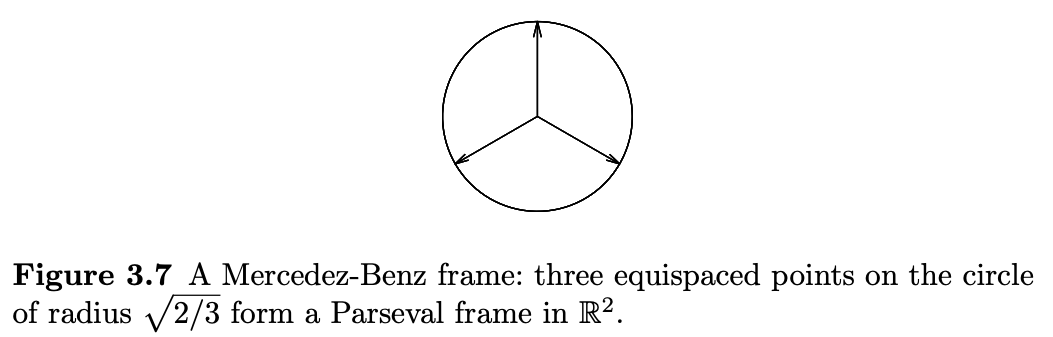
\includegraphics[width=0.8\textwidth]{Chapter 3/fig3-7.png}
\end{center}
\end{example}

Here are two more examples of isotropic distributions:

\begin{example}[Uniform on the discrete cube]
\label{ex:3.3.14}
Let $X$ be a Rademacher random vector, that is, 
\[ X \sim \mnathrm{Unif}(\{-1, 1\}^n). \]
Then $X$ is isotropic.
\end{example}

\begin{example}[Product distributions]
\label{ex:3.3.15}
Any random vector $X = (X_1, \dots, X_n)$ whose coordinates $X_i$ are independent random variables with zero 
mean and unit variance is isotropic. 
\end{example}



% ----------3.4----------
\subsection{Subgaussian Distributions in High Dimensions}
\begin{definition}[]
\label{def:3.4.1}
A random vector $X$ in $\mathbb{R}^n$ is called \underline{subgaussian} if the one-dimensional marginals 
$\left\langle X, v \right\rangle$ are subgaussian random variables for all $v \in \mathbb{R}^n$. 

The \underline{subgaussian norm} of $X$ is defined by taking the maximal subgaussian norm of the marginals 
over all unit vectors: 
\[ \lVert X \rVert_{\psi_2} = \sup_{v \in S^{n - 1}} \lVert \left\langle X, v \right\rangle \rVert_{\psi_2}. \]
\end{definition}

Below are some examples :)

\subsubsection{Gaussian, Rademacher, and More}
\begin{lemma}[Distributions with independent subgaussian coordinates]
\label{lem:3.4.2}
Let $X = (X_1, \dots, X_n)$ be a random vector in $\mathbb{R}^n$ with independent, mean zero, subgassian 
coordinates $X_i$. Then $X$ is a subgaussian random vector, and 
\[ \max_{i \leq n} \lVert X_i \rVert_{\psi_2} \leq \lVert X \rVert_{\psi_2} 
\leq C \max_{i \leq n} \lVert X_i \rVert_{\psi_2}. \]
\end{lemma}

\begin{proof}
The lower bound comes from picking $v$ as a standard basis vector in \cref{def:3.4.1}. 

For the upper bound, fix any $v = (v_1, \dots, v_n) \in S^{n - 1}$. Then 
\begin{align*}
	\lVert \left\langle X, v \right\rangle \rVert_{\psi_2}^2 
	&= \lVert \sum_{i = 1}^{n} v_i X_i \rVert_{\psi_2}^2 \\ 
	&\leq C \sum_{i = 1}^{n} \lVert v_i X_i \rVert_{\psi_2}^2 \quad \text{By \cref{prop:2.7.1}} \\
	&= C \sum_{i = 1}^{n} v_i^2 \lVert X_i \rVert_{\psi_2}^2 \\
	&\leq C \max_{i \leq n} \lVert X_i \rVert_{\psi_2}^2.
\end{align*}
Since $v$ is arbitrary, the proof is complete.
\end{proof}

\begin{example}[Rademacher]
\label{ex:3.4.3}
We can immediately get from the above that a Rademacher normal random vector is subgaussian, and 
\[ c_1 \leq \lVert X \rVert_{\psi_2} \leq c_2 \]
where $c_1, c_2 > 0$ are absolute constants.
\end{example}

\begin{example}[Normal]
\label{ex:3.4.4}
We can also get from the above that if $X \sim N(0, I_n)$, then $X$ is subgaussian. Moreover, 
$Y \sim N(0, \Sigma)$ is also subgaussian (Exercise 3.38).
\end{example}


\subsubsection{Uniform on the Sphere}
The projective CLT (\cref{thm:3.3.9}) tells us that the uniform distribution on $\sqrt{n}S^{n - 1}$ has 
approximately Gaussian 1D marginals. In fact, these marginals ar subgaussian:

\begin{theorem}[Uniform distribution on the sphere is subgaussian]
\label{thm:3.4.5}
Let $X \sim \mathrm{Unif}(S^{n - 1})$. Then for any $v \in S^{n - 1}$ and $t \geq 0$, we have 
\[ P(\left\langle X, v \right\rangle \geq t) \leq 2\exp{\left( -\frac{t^2 n}{2} \right)}. \]
In particular, $X$ is subgaussian, and $\lVert X \rVert_{\psi_2} \leq C / \sqrt{n}$.
\end{theorem}

\begin{proof}
By rotational invariance, we can assume 
\[ X = \frac{g}{\lVert g \rVert_{2}} \text{ where } g \sim N(0, I_n). \]
Again, the distribution of $\left\langle X, v \right\rangle$ does not depend on $v$ hence we can choose 
$v = e_1$ to get $\left\langle X, v \right\rangle = X_1$.

This the inequality $\left\langle X, v \right\rangle \geq t$ becomes $g_1 \geq t \lVert g \rVert_{2}$. 
By squaring both sides, moving $g_1^2$ to the LHS and simplifying, we get 
\[ g_1 \geq s \lVert \bar{g} \rVert_{2}, \quad s = \frac{t}{\sqrt{1 - t^2}} \text{ and } 
\bar{g} = (g_2, \dpts, g_n). \]

To find the probability of the event above, we fix $\lVert \bar{g} \rVert_{2}$ by conditioning on $\bar{g}$, 
which does not alter the distribution of $g$ since $g$ and $\bar{g}$ are independent. Then we uncondition 
by taking the expectation over $\bar{g}$. By the tower property, 
\[ P(\left\langle X, v \right\rangle \geq t) 
= P(g_1 \geq s \lVert \bar{g} \rVert_{2}) = \mathbb{E}[P(g_1 \geq s \lVert \bar{g} \rVert_{2}) \ | \ \bar{g}] 
\quad (*). \]

After conditioning, the conditional probability above reduces to a gaussian tail. By exercise 2.6, 
we get that 
\[ \mathbb{E}[P(g_1 \geq s \lVert \bar{g} \rVert_{2}) | \bar{g}] 
\leq \mathbb{E}[\exp{\left( -\frac{s^2 \lVert g \rVert_{2}^2}{2} \right)}] 
= \left[ \mathbb{E}[\exp{\left( -\frac{s^2 g_1^2}{2} \right)}] \right]^{n - 1}. \]
where the last equality comes from the fact that $g_i$ are i.i.d. $N(0, 1)$ random variables, and 
\[ \lVert \bar{g} \rVert_{2}^2 = g_2^2 + \cdots + g_n^2. \]
For the expression above, 
\begin{align*}
	\mathbb{E}[\exp{(-s^2 g_1^2 / 2)}] 
	&= \int_{-\infty}^{\infty} \exp{(-s^2 x^2 / 2)} \cdot 
	\frac{1}{\sqrt{2 \pi}} e^{-x^2 / 2} \ dx \\
	&= \int_{-\infty}^{\infty} \frac{1}{\sqrt{2 \pi}} \exp{\left( -\frac{(\sqrt{1 + s^2}x)^2}{2} \right)} \ dx \\
	&= \frac{1}{\sqrt{1 + s^2}} \int_{-\infty}^{\infty} e^{-v^2 / 2} \ dv \quad (v = \sqrt{1 + s^2}x) \\
	&= \frac{1}{\sqrt{1 + s^2}}.
\end{align*}
Thus the expression above becomes 
\[ \left( \frac{1}{1 + s^2} \right)^{\frac{n - 1}{2}} = (1 - t^2)^{\frac{n - 1}{2}} 
\leq \exp{\left( -\frac{t^2(n - 1)}{2} \right)} \]
since $1 - x \leq e^{-x}$ for all $x \in \mathbb{R}$. 

For the expression (*), the probability is zero for $t \geq 1$ since $\left\langle X, v \right\rangle \leq 
\lVert X \rVert_{2} \lVert v \rVert_{2} = 1$, while for $t \leq 1$, 
\[ \exp{(-t^2(n - 1) / 2)} \leq e^{1/2}\exp{(-t^2 n / 2)} \leq 2\exp{(-t^2 n / 2)} \]
and we are done.
\end{proof}

\subsubsection{Non-examples}
Some distributions in $\mathbb{R}^n$ are subgaussian, but their subgaussian norm is huge, therefore it is 
impractical to work with them. Below are a few examples.

\begin{example}[Uniform on a convex body]
\label{ex:3.4.6}
Let $K \subset \mathbb{R}^n$ be convex, and $X \sim \mathrm{Unif}(K)$ be isotropic. Qualitatively, $X$ is 
subgaussian since $K$ is bounded. But quantitatively what is it like? Is it bounded by some constant $C$?

This is true for some isotropic convex bodies like the unit cube $[-1, 1]^n$ (\cref{lem:3.4.2}) and 
the Euclidean ball of radius $\sqrt{n + 2}$ (Exercise 3.25 \& 3.42). However, for other convex bodies like the 
ball in the $ell^1$ norm, the subgaussian norm can grow with $n$ (Exercise 3.44).

Even so, a weaker result holds: $X$ has subexponential marginals, and 
\[ \lVert \left\langle X, v \right\rangle \rVert_{\psi_1} \leq C \]
for all unit vectors $v$, which comes from C. Borell's lemma, which follows from the Brunn-Minkowski inequality.
\end{example}

\begin{example}[Coordinate distribution]
\label{ex:3.4.7}
Let $X \sim \mathrm{Unif}\{\sqrt{n}e_1, \dots, \sqrt{n}e_n\}$. $X$ is subgaussian as it takes on finitely 
many values. However, from Exercise 3.43, 
\[ \lVert X \rVert_{\psi_2} \asymp \sqrt{\frac{n}{\log{n}}}. \]
Therefore it is not useful to think of $X$ as subgaussian.
\end{example}

\begin{example}[Discrete distributions]
\label{ex:3.4.8}
Some isotropic discrete distributions have subgaussian norm bounded by a constant, like the Rademacher 
distribution. However, they must take exponentially many values (Exercise 3.46). In particular, this prevents 
frames (\cref{prop:3.3.11}) as good subgaussian distributions as they take way too many values and are mostly 
useless in practice.
\end{example}


% ----------3.5----------
\subsection{Application: Grothendieck Inequality and Semidefinite Programming}
In this section, we will used high-dimensional Gaussians to tackle problems that are seemingly not related 
to probability at all. We first present the Grothendieck inequality.

\begin{theorem}[Grothendieck inequality]
\label{thm:3.5.1}
Consider $a \in \mathbb{R}^{m \times n}$. Assume that 
\[ \left| \sum_{i, j}^{} a_{ij} x_i y_j \right| \leq 1 \text{ for any numbers } x_i, y_j \in \{-1, 1\}. \]
Then for any Hilbert space $H$, we have 
\[ \left| \sum_{i, j}^{} a_{ij} \left\langle u_i, v_j \right\rangle \right| \leq K \text{ for any unit 
vectors } u_i, v_j \in H. \]
Here $K \leq 1.783$ is an absolute constant.
\end{theorem}

There is nothing random in the statement above, but we'll approach it using probabilistic reasoning. In fact, 
there will be two proofs for Grothendieck inequality, one with a much worse bound of $K \leq 14.1$ in this 
section, and the other one with $K \leq 1.783$ in section 3.7. Before going into the first argument, 
there is a simple observation that we state here.

\begin{remark}[Homogeneous form of Grothendieck inequality]
\label{rmk:3.5.2}
The assumption of Grothendieck inequality can be equivalently stated as 
\[ \left| \sum_{i, j}^{} a_{ij}x_iy_j \right| \leq \max_{i}|x_i| \cdot \max_{j}|y_j| \]
for any real numbers $x_i$ and $y_j$ (Exercise 3.47). The conclusion of Grothendieck inequality can be 
equivalently stated as
\[ \left| \sum_{i, j}^{} a_{ij} \left\langle u_i, v_j \right\rangle \right| 
\leq K \max_{i} \lVert u_i \rVert_{} \cdot \max_{j} \lVert v_j \rVert_{} \]
for any Hilbert space $H$ and any vectors $u_i, v_j, \in H$ via rescaling.
\end{remark}

\begin{proof}[Proof of \cref{thm:3.5.1} with worse bound]
(\textbf{Step 1: Reductions}) Note that Grothendieck inequality becomes trivial if we allow the value of $K$ to 
depende on the matrix $A = (a_{ij})$. For example, $K = \sum_{i, j}^{} |a_{ij}|$ would work! Let $A(K)$ be the 
smallest number that makes the conclusion in \cref{rmk:3.5.2} holds for a given matrix $A$ and any Hilbert 
space $H$ and any vectors $u_i, v_j \in H$. Our goal is to show that $K$ is actually \textit{independent} of 
both the matrix $A$ and the dimensions $m$ and $n$.

WLOG, we may show this for a specific Hilbert space $H$, namely for $\mathbb{R}^N$ equipped with the Euclidean 
norm $\lVert \cdot \rVert_{2}$. This is because we can replace $H$ with the subspace spanned by the vectors 
$u_i$ and $v_j$, which has dimension at most $N = m + n$ and inherits the norm from $H$. Then, we use the fact 
that all $N$-dimensional Hilbers spaces are isometric to $\mathbb{R}^N$ with the usual Euclidean norm 
$\lVert \cdot \rVert_{2}$. This isometry can be built by matching a given orthonormal basis of $H$ with the 
canonical bases of $\mathbb{R}^N$.

By the definition of $K = K(A)$, there exist vectors $u_i, v_j \in \mathbb{R}^N$ satisfying 
\[ \sum_{i, j}^{} a_{ij}\left\langle u_i, v_j \right\rangle = K, \ 
\lVert u_i \rVert_{2} = \lVert v_j \rVert_{2} = 1. \]

(\textbf{Step 2: Introducing randomness}) The key idea of the proof is to express the vectors $u_i, v_j$ 
using Gaussian random variables 
\[ U_i := \left\langle g, u_i \right\rangle \text{ and } V_j := \left\langle g, v_j \right\rangle, 
\text{ where } g \sim N(0, I_N). \]
Then $U_i$ and $V_j$ are standard normal random variables whose correlations follow exactly the inner products 
of the vectors $u_i$ and $v_j$ (\cref{cor:3.3.2} and Exercise 3.9):
\[ \mathbb{E}\left[ U_iV_j \right] = \left\langle u_i, v_j \right\rangle. \]
Thus 
\[ K = \sum_{i, j}^{}a_{ij} \left\langle u_i, v_j \right\rangle 
= \mathbb{E}\left[ \sum_{i, j}^{}a_{ij}U_iV_j \right] \quad (*). \]

Suppose for a moment that the random variables $|U_i|$ and $|V_j|$ were to be almost surely bounded by some 
constant, say $R$. Then from the assumption in \cref{rmk:3.5.2}, 
\[ \left| \sum_{i, j}^{} a_{ij}U_iV_j \right| \leq R^2 \text{ almost surely. } \]
Plugging this into the equation above will give $K \leq R^2$, completing the proof.

(\textbf{Step 3: Truncation}) The above is flawed, because the Gaussian random variables $U_i, V_j$ are 
unbounded. But their tails are light enough that they are close to being bounded. To act on this heuristic, we 
use a \textit{truncation} trick. Pick a level $R \geq 1$ and split the random variables like this:
\[ U_i = U_i^- + U_i^+ \text{ where } U_i^- = U_i \mathbf{1}_{\{|U_i| \leq R\}} \text{ and } 
U_i^+ = U_i \mathbf{1}_{\{|U_i| > R\}}. \]
We similarly decompose $V_j = V_j^- + V_j^+$. Nor $U_i^-$ and $V_j^-$ are bounded by $R$, as desired. The 
remainder terms $U_I^+$ and $V_j^+$ are small in the $L^2$ norm: by Exercise 2.4 (b), a Gaussian tail bound 
gives 
\[ \lVert U_i^+ \rVert_{L^2}^2 \leq 2 \left( R + \frac{1}{R} \right) \frac{1}{\sqrt{2 \pi}}e^{-R^2 / 2} 
< \frac{4}{R^2} \quad (**). \]
A similar bound holds for $V_j^+$.

(\textbf{Step 4: Breaking up the sum}) Replacing $U_i V_j$ with $(U_i^- + U_i^+)(V_j^- + V_j^+)$ in $(*)$ and 
expanding the sum, we get 
\[ K = \underbrace{\mathbb{E}\left[ \sum_{i, j}^{} a_{ij} U_i^- V_j^- \right]}_{S_-}
+ \underbrace{\mathbb{E}\left[ \sum_{i, j}^{} a_{ij} U_i^+ V_j^- \right]}_{S_{\pm}}
+ \underbrace{\mathbb{E}\left[ \sum_{i, j}^{} a_{ij} U_i^- V_j^+ \right]}_{S_{\mp}} 
+ \underbrace{\mathbb{E}\left[ \sum_{i, j}^{} a_{ij} U_i^+ V_j^+ \right]}_{S_+}. \]
Let's bound each term! $S_-$ is the easiest to bound: by construction, $|U_i|$ and $|V_j|$ are bounded by $R$, 
so from step 2 we can directly get that 
\[ S_- \leq R^2. \]

We cannot use the same reasoning for $S_{\pm}$, since the random variable $U_i^+$ is unbounded. Instead, let 
us treat the random variables $U_i^+$ and $V_j^-$ as elements of the Hilbert space $L^2$ with the inner product 
$\left\langle X, Y \right\rangle_{L^2} = \mathbb{E}\left[ XY \right]$. Thus write 
\[ S_{\pm} = \sum_{i, j}^{} a_{ij} \left\langle U_i^+, V_j^- \right\rangle_{L^2}. \]
We have $\lVert U_i^+ \rVert_{L^2} < 2/R$ by $(**)$, and $\lVert V_j^- \rVert_{L^2} \leq 
\lVert V_j \rVert_{L^2} = 1$ by construction. Then, applying the conclusion from \cref{rmk:3.5.2} for the 
Hilbert space $H = L^2$, we find that 
\[ S_{\pm} = K \cdot \frac{2}{R}. \]
(It might seem odd that we are using the inequality that we are trying to prove. However, we picked 
$K = K(A)$ at that start to be the smallest value to make Grothendieck inequality work. That is the $K$ that 
we are using here).

The last two terms, $S_{\mp}$ and $S_+$, can be bounded just like the above (Check).

(\textbf{Step 5: Putting everything together}) Plugging the bounde on all four terms, we conclude that 
\[ K \leq R^2 + \frac{6K}{R}. \]
Setting $R = 12$ and rearranging the terms gives $K \leq 288$. A litte finer analysis, skipping the rough 
$4 / R^2$ bound in $(**)$ yields $K \leq 14.1$ (Exercise 3.48).
\end{proof}

\begin{remark}[Quadratic Grothendieck]
\label{rmk:3.5.3}
We can often relax Grothendieck inequality by taking $x_i = y_i$, bounding a quadratic instead of a bilinear 
form. The statement becomes: Let $A \in \mathbb{R}^{n \times n}$ be symmetric PSD or diagonal-free. Assume that 
\[ \left| \sum_{i, j}^{} a_{ij}x_ix_j \right| \leq 1 \text{ for any numbers } x_i \in \{-1, 1\}. \]
Then for any Hilbert space $H$, we have 
\[ \left| \sum_{i, j}^{} a_{ij}\left\langle u_i, v_j \right\rangle \right| \leq 2K \text{ for any unit vectors} 
u_i, v_j \in H. \]
Here $K$ is the the absolute constant from Grothendieck inequality.
\end{remark}

\begin{proof}
Exercises 3.49 \& 3.50.
\end{proof}


\subsubsection{Semidefinite Programming}
Some hard computational problems can be relazed into easier, more computationally tractable programs via 
semidefinite programming, and Grothendieck inequality can help guarantee its quality.

\begin{definition}[]
\label{def:3.5.4}
A \underline{semidefinite program (SDP)} is an optimization problem of the following type: 
\[ \text{maximize } \left\langle A, X \right\rangle: \ X \succeq 0, \ 
\left\langle B_i, X \right\rangle \leq b_i \text{ for } i = 1, \dots, N. \]
\end{definition}
Here $A, B$ are given $n \times n$ matrices, and $b_i$ are given numbers. The variable $X$ is an $n \times n$ 
symmetric PSD matrix, indicated by the notation $X \succeq 0$. The inner product is the standard one on the 
space of $n \times n$ matrices: 
\[ \left\langle A, X \right\rangle = \mathrm{tr}(A^T X) = \sum_{i, j = 1}^{n}A_{ij}X_{ij}. \]
Note that if we \textit{minimize} instead of maximize, we still get a semidefinite program. Same goes for 
replacing any signs ``$\leq$" by ``$\geq$" or ``$=$".

\begin{remark}[An SDP program is a convex program]
\label{rmk:3.5.5}
Every SDP is a convex program because it involves maximizing a \textit{linear} function $\left\langle A, X 
\right\rangle$ over a convex set of matrices (the set of PSD matrices is convex, and so is its intersection 
with the half-spaces defined by the constraints $\left\langle B_i, X \right\rangle \leq b_i$). This is good news 
because convex programs are \textit{algorithmically tractable}, i.e. there are efficient solvers for general 
convex programs, and specifically for SDPs.
\end{remark}

\begin{center}
	\textit{Semidefinite Relaxations}
\end{center}

SDPs can provide efficient relaxations of computationally hard problems, such as 
\[ \text{maximize } \sum_{i, j = 1}^{n}A_{ij}x_ix_j: \ x_i = \pm 1 \text{ for } i = 1, dots, n \]
where $A$ is a given $n \times n$ matrix. This is a \textit{quadratic integer optimization problem}, whose 
feasible set consists of $2^n$ vectors $x \in \{-1, 1\}^n$. Finding the maximum via brute force takes 
exponential time. Moreover, there is probably not a smarter way because it is a computationally hard problem 
(NP-hard).

However, we can relax the problem into a SDP program than approximates the maximum within a constant factor. 
To do this, we replace the numbers $x_i = \pm 1$ by random variables $X_i$ in $\mathbb{R}^n$. We get 
\[ \text{maximize } \sum_{i, j = 1}^{n}A_{ij}\left\langle X_i, X_j \right\rangle: 
\ \lVert X_i \rVert_{2} = 1 \text{ for } i = 1, \dots, n. \]

\begin{proposition}[The relaxation is an SDP]
\label{prop:3.5.6}
The optimization problem above is equivalent to the following SDP:
\[ \text{maximize } \left\langle A, Z \right\rangle: \ Z \succeq 0, Z_{ii} = 1 \text{ for } i = 1, \dots, n. \]
\end{proposition}

\begin{proof}
Recall that the \underline{Gram matrix} of vectors $X_1, \dots, X_n$ is the $n \times n$ matrix $Z$ with entries 
$Z_{ij} = \left\langle X_i, X_j \right\rangle$. Then the two problems are equivalent thanks to two linear 
algebra facts: (a) the Gram matrix of any set of vectors is symmetric and PSD, and (b) conversely, any 
symmetric PSD matrix is a Gram matric of some set of vectors (Exercise 3.51).
\end{proof}

\begin{center}
	\textit{The guarantee of relaxation}
\end{center}

Let's show that the probabilistic SDP approximates the exact SDP within a constant factor:

\begin{theorem}[]
\label{thm:3.5.7}
Let $A \in \mathbb{R}^{n \times n}$ be symmetric PSD. Let $\mathrm{\int}(A)$ denote the maximum in the integer 
optimization problem, and $\mathrm{sdp}(A)$ denote the maximum in the probabilistic SDP. Then 
\[ \mathrm{\int}(A) \leq \mathrm{sdp}(A) \leq 2K \cdot \mathrm{\int}(A) \]
where $K \leq 1.783$ is the constant in Grothendieck inequality.
\end{theorem}

\begin{proof}
The first bound follows with $X_i = (x_i, 0, \dots, 0)^T$. The second comes directly from the quadratic 
Grothendieck inequality in \cref{rmk:3.5.3}.
\end{proof}

Although \cref{thm:3.5.7} helps us approximate the maximum value in the integer SDP, it is not obvious how to 
find the actual solution that attain this maximum value. Can we convert the vectors $X_i$ that give a solution 
to the probabilistic SDP into labels $x_i = \pm 1$ that approximately solve the integer SDP?

The answer is yes! But we need some knowledge of max-cuts first. After reading, we can create an even better 
approximation constant than $2K$ (Exercise 3.58).



% ----------3.6----------
\subsection{Application: Maximum Cut for Graphs}
Semidefinite relaxations can be useful for tackling one of the well known NP-hard problems: finding the maximum 
cut of a graph.

An undirected graph $G = (V, E)$ is defined as a set of vertices $V$ together with a set of edges $E$; each 
edge is an unordered pair of vertices. We focus on finite, simple graphs - no loops or multiple edges. For 
convenience, label the vertices by integers, setting $V = \{1, \dots, n\}$.

\begin{definition}[]
\label{def:3.6.1}
If we partition th evertices of a graph $G$ into two disjoint subsets, the \underline{cut} is the number of 
edges between them. Then \underline{maximum cut} of $G$, denoted $\mathrm{maxcut}(G)$, is the largest possible 
cut over all partitions of vertices. The figure below is an illustration:
\begin{center}
	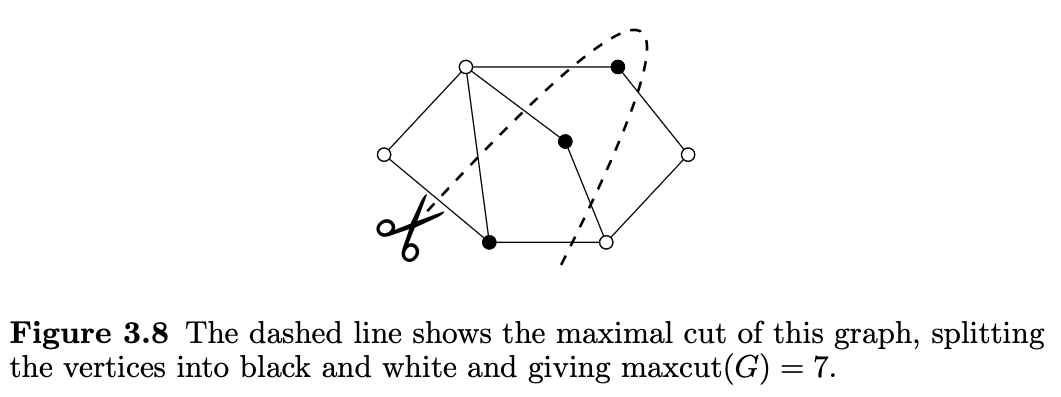
\includegraphics[width=0.8\textwidth]{Chapter 3/fig3-8.png}
\end{center}
\end{definition}
Finding the maximum cut is generally a computationally hard problem (NP-hard).


\subsubsection{A Simple 0.5-approximation Algorithm}
We can relax the maximum cut problem into a SDP, but we have to translate the problem into linear algebra first.

\begin{definition}[]
\label{def:3.6.2}
The \underline{Adjacency matrix} $A$ of a graph $G$ with vertices $V = \{1, \dots, n\}$ is a symmetric 
$n \times n$ matrix where $A_{ij} = 1$ if vertices $i$ and $j$ are connected by an edge, and $A_{ij} = 0$ 
otherwise.
\end{definition}

A partition of the vertices into two sets can be described by a vector of labels 
\[ x = (x_i) \in \{-1, 1\}^n \]
where the sign of $x_i$ shows which subset $x_i$ belongs to. For example, in Figure 3.8 from above, the three 
black vertices might have $x_i = 1$ and the four white vertices $x_i = -1$. The cut for $G$ for this partition 
is simply the number of edges between vertices with opposite labels:
\[ \mathrm{cut}(G, x) = \frac{1}{2}\sum_{i, j: x_ix_j = -1}^{} A_{ij} 
= \frac{1}{4} \sum_{i, j = 1}^{n} A_{ij}(1 - x_ix_j). \]
The maximum cut is found by maximizing $\mathrm{cut}(G, x)$ over all partitions $x$: 
\[ \mathrm{maxcut}(G) = \frac{1}{4} \max_{}\left\{ \sum_{i, j = 1}^{n} A_{ij}(1 - x_ix_j): \ x_i = \pm 1 
\forall i\right\}. \]
Let's start with a simple 0.5-approximation algorithm for the maximum cut - one that finds a vut with at least 
half of the edges of $G$.

\begin{proposition}[0.5-approximation algorithm for maximum cut]
\label{prop:3.6.3}
If we split the vertices of $G$ into two sets at random, uniformly over all $2^n$ partitions, the expected cut 
is at least $0.5 \mathrm{maxcut}(G)$.
\end{proposition}

\begin{proof}
A random cut is generated by a Rademacher random vector $x$. Then, in the formula for $\mathrm{cut}(G, x)$ 
we hvae $\mathbb{E}\left[ x_ix_j \right] = 0$ for $i \neq j$ and $A_{ij} = 0$ for $i = j$ since the graph has 
no loops. Thus, by linearity of expectation, 
\[ \mathbb{E}\left[ \mathrm{cut}(G, x) \right]
= \frac{1}{4} \sum_{i, j = 1}^{n} A_{ij} = \frac{1}{2}|E| \geq \frac{1}{2}\mathrm{maxcut}(G). \]
\end{proof}


\subsubsection{Semidefinite Relaxation}
We can get a 0.878-approximation algorithm due to Goemans and Williamson. It is based on a semidefinite 
relaxation of the NP-hard problem. We consider the SDP 
\[ \mathrm{sdp}(G) := \frac{1}{4} \max_{}\left\{ \sum_{i, j = 1}^{n} A_{ij} 
(1 - \left\langle X_i, X_j \right\rangle): \ X_i \in \mathbb{R}^n, \ \lVert X_i \rVert_{2} = 1 \ 
\forall i \right\}. \]

We'll show that the $\mathrm{sdp}(G)$ approximates $\mathrm{maxcut}(G)$ within a 0.878 factor, and how to turn 
the solution $(X_i)$ into labels $x_i = \pm 1$ for an actual partition of the graph. We do this by 
\textit{randomized rounding}: Pick a random hyperplane through the origin in $\mathbb{R}^n$ and assign $x_i = 1$ 
to the vectors $X_i$ on one side, $x_i = -1$ to the other (see figure below). More formally, consider a standard 
normal random vector $g \sim N(0, I_n)$ and define 
\[ x_i := \mathrm{sign}\left\langle X_i, g \right\rangle, \ i = 1, \dots, n. \]

\begin{center}
	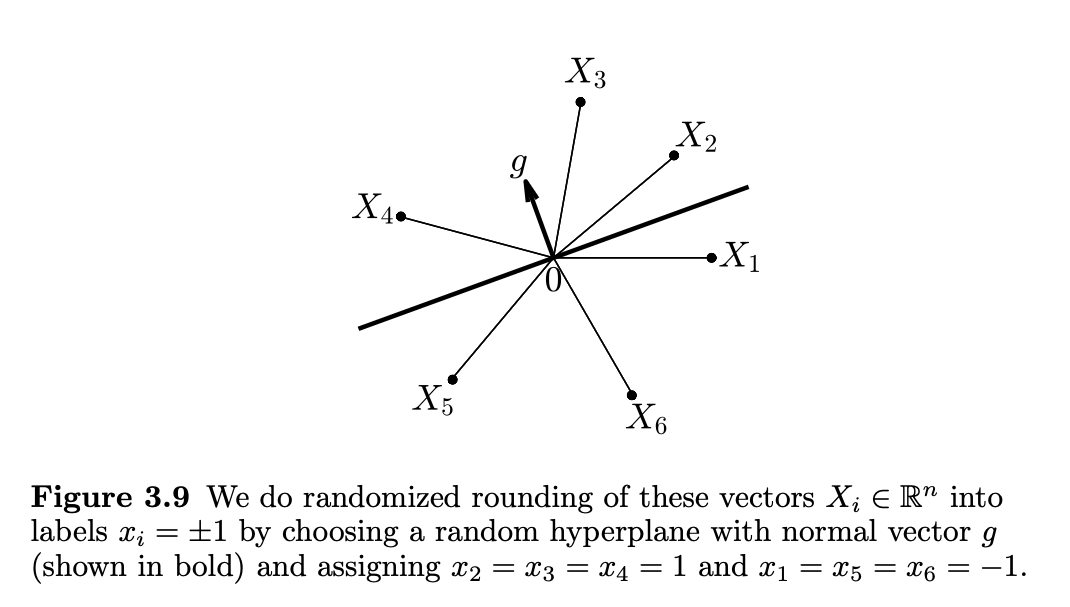
\includegraphics[width=0.8\textwidth]{Chapter 3/fig3-9.png}
\end{center}

\begin{theorem}[]
\label{thm:3.6.4}
Let $G$ be a graph with adjacency matrix $A$. Let $(X_i)$ be a solution of the SDP, and $x = (x_i)$ be the 
result of a randomized rounding of $(X_i)$. Then 
\[ \mathbb{E}\left[ \mathrm{cut}(G, x) \right] \geq 0.878 \mathrm{sdp}(G) \geq 0.878 \mathrm{maxcut}(G). \]
\end{theorem}

The proof is based on an elementary inequality. In proving Grothendieck inequality (\cref{thm:3.5.1}), we 
relied on the fact that if $g \sim N(0, I_n)$ then 
\[ \mathbb{E}\left[ \left\langle g, u \right\rangle \left\langle g, v \right\rangle \right] 
= \left\langle u, v \right\rangle \]
for any fixed vectors $u, v \in \mathbb{R}^n$ (Exercise 3.9). We will need a slightly more advanced version of 
this identity:

\begin{lemma}[Grothendieck identity]
\label{lem:3.6.5}
Consider a random vector $g \sim N(0, I_n)$. Then for any fixed vectors $u, v \in S^{n - 1}$, we have 
\[ \mathbb{E}\left[ \mathrm{sign}\left\langle g, u \right\rangle \mathrm{sign}\left\langle g, v 
\right\rangle \right] = \frac{2}{\pi} \arcsin{\left\langle u, v \right\rangle}. \]
\end{lemma}

\begin{proof}
Exercise 3.53.
\end{proof}

A downside of the Grothendieck inequality is the nonlinear function arcsin, which is hard to work with. We can 
replace it with a linear bound using the inequality 
\[ 1 - \frac{2}{\pi}\arcsin{t} = \frac{2}{\pi} \arccos{t} \geq 0.878(1 - t), t \in [-1, 1]. \]
which can be checked easily with software (shown below).

\begin{center}
	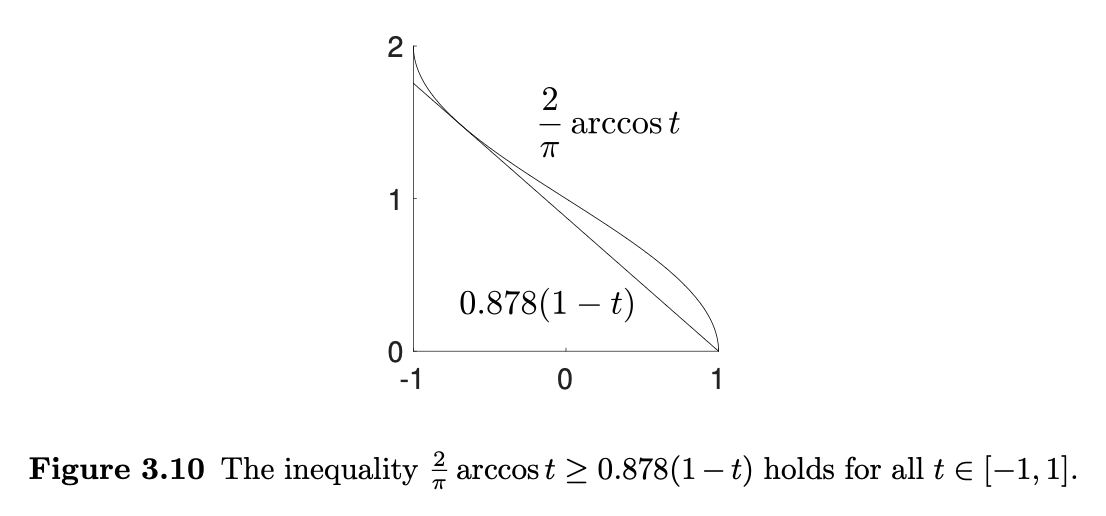
\includegraphics[width=0.8\textwidth]{Chapter 3/fig3-10.png}
\end{center}

\begin{proof}[Proof of Theorem 3.6.4]
By the formula for $\mathrm{cut}(G, x)$ and linearity of expectation, we have 
\[ \mathbb{E}\left[ \mathrm{cut}(G, x) \right] = \frac{1}{4}\sum_{i, j = 1}^{n}
A_{ij}(1 - \mathbb{E}\left[ x_ix_j \right]). \]
The definiton of the labels $x_I$ in the rounding step gives 
\begin{align*}
	1 - \mathbb{E}\left[ x_ix_j \right] 
	&= 1 - \mathbb{E}\left[ \mathrm{sign}\left\langle X_i, g \right\rangle 
	\mathrm{sign}\left\langle X_j, g \right\rangle \right] \\
	&= 1 - \frac{2}{\pi}\arcsin{\left\langle X_i, X_j \right\rangle} \quad \text{(\cref{lem:3.6.5})} \\
	&\geq 0.878(1 - \left\langle X_i, X_j \right\rangle).
\end{align*}
Therefore 
\[ \mathbb{E}\left[ \mathrm{cut}(G, x) \right] 
\geq 0.878 \cdot \frac{1}{4} \sum_{i, j = 1}^{n} A_{ij}(1 - \left\langle X_i, X_j \right\rangle) 
= 0.878 \mathrm{SDP}(G). \]
This proves the first inequality. The second inequality is trivial since $\mathrm{sdp}(G) 
\geq \mathrm{maxcut}(G)$.
\end{proof}



% ----------3.7----------
\subsection{Kernel Trick and Tightening of Grothendieck Inequality}
This section takes a different approach to the proof of Grothendieck inequality for (almost) the best known 
bound: $K \leq 1.783$.

We'll again use Grothendieck identity (\cref{lem:3.6.5}), but the nonlinearity of the arcsin function is a big 
challenge. If there were no nonlinearity, we would have
\[ \mathbb{E}\left[ \mathrm{sign}\left\langle g, u \right\rangle 
\mathrm{sign}\left\langle g, v \right\rangle \right] = \frac{2}{\pi}\left\langle u, v \right\rangle, \]
of which Grothendieck inequality would easily follow:
\[ \frac{2}{\pi}\sum_{i, j}^{}a_{ij}\left\langle u_i, v_j \right\rangle 
= \mathbb{E}\left[ \sum_{i, j}^{}a_{ij}\mathrm{sign}\left\langle g, u_i \right\rangle 
\mathrm{sign}\left\langle g, v_j \right\rangle \right] \leq 1. \]
This would give $K \leq \pi / 2 \approx 1.57$.

The above is obviously wrong because of nonlinearity. To handle the nonlinear function, of an inner product 
$\left\langle u, v \right\rangle$, we can use a remarkably powerful trickL rewrite it as a (linear) inner 
product $\left\langle u', v' \right\rangle$ for some other vectors $u', v'$ in some Hilbert space $H$. In the 
literature of machine learning, this is known as the \textit{kernel trick}.

We will explicitly construct the nonlinear transformations $u' = \Phi(u)$, $v' = \Psi(v)$ that will do the job. 
The best way to describe them is to use tensors, which generalize matrices to higher dimensions.


\subsubsection{Tensors}
\begin{definition}[]
\label{def:3.7.1}
An \underline{order $k$ tensor} $(a_{i_1 \dots i_k})$ is an $n_1 \times n_2 \times \cdots \times n_k$ array 
of real numbers $a_{i_1 \dots i_k}$. The canonical inner product on $\mathbb{R}^{n_1 \times \cdots \times n_k}$ 
defines the inner product of tensors: For $A, B$ tensors (of the same dimensions), 
\[ \left\langle A, B \right\rangle := \sum_{i_1, \dots, i_k}^{} a_{i_1 \dots i_k} b_{i_1 \dots i_k}. \]
\end{definition}

\begin{example}[Vectors and matrices]
\label{ex:3.7.2}
Vectors are order 1 tensors, and matrices are order 2 tensors. The inner product for tensors generalized the 
inner product for vectors and matrices.
\end{example}

\begin{example}[Rank-one tensors]
\label{ex:3.7.3}
For a vector $u \in \mathbb{R}^n$, the order $k$ tensor product $u \otimes \cdots \otimes u$ is the tensor whose 
entries are the products of all $k$-tuples of the entries of $u$:
\[ u \otimes \cdots \otimes u = u^{\otimes k} := (u_{i_1} \cdots u_{i_k}) \in 
\mathbb{R}^{n \times \cdots \times n}. \]
For example, if $k = 2$, the tensor product $u \otimes u$ is the $n \times n$ matrix 
\[ u \otimes u = (u_iu_j)_{i, j = 1}^n = uu^T. \]
\end{example}

\begin{lemma}[Powers]
\label{lem:3.7.4}
For any vectors $u, v \in \mathbb{R}^n$ and $k \in \mathbb{N}$, we have 
\[ \left\langle u^{\otimes k}, v^{\otimes k} \right\rangle = \left\langle u, v \right\rangle^k. \]
\end{lemma}

\begin{proof}
For $n = 3$: 
\begin{align*}
	\left\langle u^{\otimes 3}, v^{\otimes 3} \right\rangle 
	&= \sum_{i, j, k = 1}^{n} (u_i u_j u_k)(v_iv_jv_k) \\
	&= \left( \sum_{i = 1}^{n}u_iv_i \right) \left( \sum_{i = 1}^{n}u_iv_i \right)
    \left( \sum_{i = 1}^{n}u_iv_i \right) \\
	&= \left\langle u, v \right\rangle^3.
\end{align*}
The general case is similar to the above.
\end{proof}

\cref{lem:3.7.4} reveals something interesting: non-linear expressions like $\left\langle u, v \right\rangle^k$ 
can be written as a stardard \textit{linear} inner product in a different space. Specifically, there is a 
Hilbert space $H$ and a transformation $\Phi: \mathbb{R}^n \to H$ such that 
\[ \left\langle \Phi(u), \Phi(v) \right\rangle = \left\langle u, v \right\rangle^k 
\text{ for any } u, v \in \mathbb{R}^n. \]
In fact we can take $H = \mathbb{R}^{n^k}$, the space of $k$-th order tensors and $\Phi(u) = u^{\otimes k}$. 

Now, we can move to general nonlinearities: 
\begin{example}[Polynomials with nonnegative coefficients]
\label{ex:3.7.5}
There exists a Hilbert space $H$ and a transformation $\Phi: \mathbb{R}^n \to H$ such that 
\[ \left\langle \Phi(u), \Phi(v) \right\rangle = 2 \left\langle u, v \right\rangle^2 
+ 5 \left\langle u, v \right\rangle^3 \text{ for all } u, v \in \mathbb{R}^n. \]
We can take 
\[ \Phi(u) = (\sqrt{2}u \otimes u) \oplus (\sqrt{5}u \otimes u \otimes u) \]
where $\oplus$ denotes concatenation. So, the target space is $\mathbb{R}^{n^2 + n^3}$.
\end{example}

\begin{example}[General polynomials]
\label{ex:3.7.6}
Polynomials with negative coefficients can make our task impossible since $\left\langle \phi(u), 
\Phi(v) \right\rangle$ is always nonnegative. But here is a neat workaround: we can find \textit{two} 
transformations, possibly different, such that 
\[ \left\langle \Phi(u), \Phi(v) \right\rangle = 2 \left\langle u, v \right\rangle^2 
- 5 \left\langle u, v \right\rangle^3 \text{ for all } u, v \in \mathbb{R}^n. \]
In this case, we can take 
\[ \Phi(u) = (\sqrt{u} \otimes u) \oplus (\sqrt{5}u \otimes u \otimes u), 
\Psi(v) = (\sqrt{2}v \otimes v) \oplus (-\sqrt{5}v \otimes v \otimes v). \]
Note that the transformations keep the lengths of vectors under control. For any unit vector $u$, 
\[ \lVert \Phi(u) \rVert_{2}^2 = \lVert \Psi(u) \rVert_{2}^2 
= 2 \left\langle u, u \right\rangle^2 + 5 \left\langle u, u \right\rangle^3 = 2 + 5 = 7, \]
which is just the sum of the absolute values of the coefficients.
\end{example}

Following this approach, we can handle any polynomial $f(x) = \sum_{k = 1}^{N} a_k x^k$. Moreover, by taking 
limits on polynomials, we can handle even more functions:

\begin{lemma}[Real analytic functions]
\label{lem:3.7.7}
Consider a function $f(x) = \sum_{k = 0}^{\infty} a_kx^k$ where the series converges for all $x \in 
\mathbb{R}$. There exists a Hilbert space $H$ and transformations $\Phi, \Psi: \mathbb{R}^n \to H$ such that 
\[ \left\langle \Phi(u), \Psi(v) \right\rangle = f(\left\langle u, v \right\rangle) \text{ for all } 
u, v \in \mathbb{R}^n. \]
Moreover, for any unit vector $u$, we have 
\[ \lVert \Phi(u) \rVert_{2}^2 = \lVert \Psi(u) \rVert_{2}^2 = \sum_{k = 0}^{\infty}|a_k|. \]
\end{lemma}

\begin{proof}
Exercise 3.55.
\end{proof}

\begin{example}[Sine function]
\label{ex:3.7.8}
Let $c > 0$. The function $f(x) = \sin{(cx)}$ is real analytic: 
\[ \sin{(cx)} = cx - \frac{(cx)^3}{3!} + \frac{(cx)^5}{5!} - \frac{(cx)^7}{7!} + \cdots \]
Thus, there exists a Hilbert space $H$ and transformations $\Phi, \Psi: \mathbb{R}^n \to H$ such that 
\[ \left\langle \Phi(u), \Psi(v) \right\rangle = \sin{(c \left\langle u, v \right\rangle )} 
\text{ for all } u, v \in \mathbb{R}^n. \]
Also, $\Phi$ and $\Psi$ map unit vectors to unit vectors if 
\[ 1 = c + \frac{c^3}{3!} + \frac{c^5}{5!} - \frac{c^7}{7!} + \cdots = \frac{e^c + e^{-c}}{2}. \]
Solving this equation yields $c = \ln{(1 + \sqrt{2})}$.
\end{example}


\subsubsection{Proof of Theorem 3.5.1}
We're going to prove Grothendieck inequality (\cref{thm:3.5.1}) with constant 
\[ K \leq \frac{\pi}{2 \ln{(1 + \sqrt{2})}} \approx 1.783. \]
We can assume WLOG that $u_i, v_j \in \mathbb{R}^N$ with $N = n + m$, just like in the proof of Grothendieck 
inequality in Section 3.5. Then, by \cref{ex:3.7.8} with $c = \ln{(1 + \sqrt{2})}$, we can find unit vectors 
$u_i', v_j'$ in some Hilbert space $H$ satisfying 
\[ \left\langle u_i', v_j' \right\rangle = \sin{(c \left\langle u_i, v_j \right\rangle)} 
\text{ for all } i, j. \]
Again, we can assume WLOG that $H = R^N$. Applying Grothendieck identity (\cref{lem:3.6.5}), we get 
\[ \mathbb{E}\left[ \mathrm{sign}\left\langle g, u_i' \right\rangle 
\mathrm{sign}\left\langle g, v_j' \right\rangle \right] 
= \frac{2}{\pi}\arcsin{\left\langle u_i', v_j' \right\rangle} 
= \frac{2c}{\pi}\left\langle u_i, v_j \right\rangle. \]
Thys 
\[ \frac{2c}{\pi} \sum_{i, j}^{}a_{ij}\left\langle u_i, v_j \right\rangle 
= \mathbb{E}\left[ \sum_{i, j}^{}a_{ij} \underbrace{\mathrm{sign}\left\langle g, u_i' \right\rangle}_{X_i}
\underbrace{\mathrm{sign}\left\langle g, v_j' \right\rangle}_{Y_i} \right] \leq 1. \]
The last step follows from the assumption of Grothendieck inequality since $X_i, Y_j \in \{-1, 1\}$. The 
proof is complete since $c = \ln{(1 + \sqrt{2})}$. $\square$

\begin{remark}[An algorithmic viewpoint]
\label{rmk:3.7.9}
This proof gives a randomized algorithm that takes a matrix $A$ and unit vectors $u_i, v_j$ and finds labels 
$x_i, y_j \in \{-1, 1\}$ satisfying 
\[ \mathbb{E}\left[ \sum_{i, j}^{}a_{ij}x_iy_j \right] \geq \frac{1}{K} \sum_{i, j}^{}a_{ij} 
\left\langle u_i, v_j \right\rangle. \]
Here is how it works: First, find unit vectors $u_i', v_j' \in \mathbb{R}^{n + m}$ with prescribed inner 
products. Then use randomized rounding: pick $g \sim N(0, I_n)$ and set $x_i = \mathrm{sign}\left\langle 
gm u_i' \right\rangle$ and $y_i = \mathrm{sign}\left\langle g, v_i' \right\rangle$.
\end{remark}


\subsubsection{Kernels and Feature Maps}
Since the kernel trick worked so well for Grothendieck inequality, we might wonder - what other nonlinearities 
can it handle? Given a function of two variables $K: \mathcal{X} \times \mathcal{X} \to \mathbb{R}$ on some 
set $\mathcal{X}$, when can we find a Hilbert space $H$ and a transformation $\Phi: \mathcal{X} \to H$ such 
that 
\[ \left\langle \Phi(u), \Phi(v) \right\rangle = K(u, v) \text{ for all } u, v \in \mathcal{X}? \quad (*) \]

The answer is given by Mercer's Theorem, and more precisely, the Moore-Aronszajn Theorem. The necessary 
and sufficient condition is that $K$ be a \textit{positive semidefinite kernel}, meaning that for any points 
$u_1, \dots, U_N \in \mathcal{X}$, the kernel matrix $(K(u_i, u_j))_{i, j = 1}^N$ has to be symmetric PSD. 
The transformation $\Phi$ is called a \textit{feature map}, and the Hilbert space $H$ is called a 
\textit{Reproducing Kernel Hilbert Space} (RKHS). 

Popular PSD kernels in machine learning include the Gaussian and polynomial kernels, given by:
\[ K(u, v) = \exp{\left( -\frac{\lVert u - v \rVert_{2}^2}{2 \sigma^2} \right)}, \ 
K(u, v) = (\left\langle u, v \right\rangle + r)^k, \ u, v \in \mathbb{R}^n, \]
where $\sigma > 0, r > 0, k \in \mathbb{N}$ are hyperparameters. The kernel trick, which expresses a kernel 
$K(u, v)$ as an inner product, is widely used in machine learning because it lets us handle nonlinear models 
(determined by $K$) with techniques designed for linear models (e.g. Kernel Ridge Regression). The exact 
details of the Hilbert space $H$ and feature map $\Phi$ are usually not needed. Moreover, to compute the inner 
product $\left\langle \Phi(u), \Phi(v) \right\rangle$ in $H$, we don't even need to know $\Phi$ - the identity 
above ($*$) let's us calculate $K(u, v)$ directly!
